%% -----------------------------------------------------------
%% Projeto 2 da disciplina de INF2608 - Fundamentos de Computação Gráfica
%% Relatório LaTeX (INÍCIO) — Path Tracing.
%% Modelado em inf2608-proj1.v3.tex (mesma classe, infra e bibliografia).
%% Cobre apenas as etapas IMPLEMENTADAS: 02 (core), 03 (NEE), 04 (MIS),
%% 05 (Russian Roulette), 06 (mesh light), 07 (dielétrico).

\documentclass[portuguese]{sbcreviews-2025}%
\usepackage[misc,geometry]{ifsym}
\usepackage{aas_macros}
\usepackage[bottom]{footmisc}
\usepackage{tabularray}
\usepackage{afterpage}
\usepackage{url}
\usepackage{pifont}
\usepackage{amsmath}

\setcitestyle{square}
\captionsetup[figure]{hypcap=false}

%% --- Slides do Prof. Celes (traçado de caminhos) ---
\newcommand{\DeclareSlideURL}[2]{\expandafter\def\csname slideurl@#1\endcsname{#2}}
\newcommand{\slideurl}[1]{%
    \ifcsname slideurl@#1\endcsname
        \csname slideurl@#1\endcsname
    \else
        #1
    \fi
}
\DeclareSlideURL{inf2608slides07}{https://github.com/yangricardo/INF2608-comp-grafica/blob/main/materiais/tra\%C3\%A7ado_de_caminhos/7.montecarlo.pdf}
\DeclareSlideURL{inf2608slides08}{https://github.com/yangricardo/INF2608-comp-grafica/blob/main/materiais/tra\%C3\%A7ado_de_caminhos/8.tracado_de_caminhos.pdf}
\DeclareSlideURL{inf2608slides09}{https://github.com/yangricardo/INF2608-comp-grafica/blob/main/materiais/tra\%C3\%A7ado_de_caminhos/9.tracado_de_caminhos2.pdf}
\newcommand{\slidescite}[2]{\citep[\href{\slideurl{#1}}{pp.~#2}]{#1}}
\newcommand{\slidesref}[3]{\href{\slideurl{#1}}{Slides #2}, pp.~#3}

%% --- Seções do PBRT 4e ---
\newcommand{\pbrtcontentsurl}{https://pbr-book.org/4ed/contents.html}
\newcommand{\DeclarePBRTSectionURL}[2]{\expandafter\def\csname pbrturl@#1\endcsname{#2}}
\newcommand{\pbrtsectionurl}[1]{%
    \ifcsname pbrturl@#1\endcsname
        \csname pbrturl@#1\endcsname
    \else
        \pbrtcontentsurl
    \fi
}
\DeclarePBRTSectionURL{2.2.3}{https://pbr-book.org/4ed/Monte_Carlo_Integration/Improving_Efficiency.html\#MultipleImportanceSampling}
\DeclarePBRTSectionURL{2.2.4}{https://pbr-book.org/4ed/Monte_Carlo_Integration/Improving_Efficiency.html\#RussianRoulette}
\DeclarePBRTSectionURL{6.5}{https://pbr-book.org/4ed/Shapes/Triangle_Meshes.html}
\DeclarePBRTSectionURL{9.2}{https://pbr-book.org/4ed/Reflection_Models/Diffuse_Reflection.html}
\DeclarePBRTSectionURL{9.5}{https://pbr-book.org/4ed/Reflection_Models/Dielectric_BSDF.html}
\DeclarePBRTSectionURL{11.2}{https://pbr-book.org/4ed/Volume_Scattering/Transmittance.html}
\DeclarePBRTSectionURL{12.4}{https://pbr-book.org/4ed/Light_Sources/Area_Lights.html}
\DeclarePBRTSectionURL{12.6}{https://pbr-book.org/4ed/Light_Sources/Light_Sampling.html}
\DeclarePBRTSectionURL{13.1}{https://pbr-book.org/4ed/Light_Transport_I_Surface_Reflection/The_Light_Transport_Equation.html}
\DeclarePBRTSectionURL{13.3}{https://pbr-book.org/4ed/Light_Transport_I_Surface_Reflection/A_Simple_Path_Tracer.html}
\DeclarePBRTSectionURL{13.4}{https://pbr-book.org/4ed/Light_Transport_I_Surface_Reflection/A_Better_Path_Tracer.html}
\DeclarePBRTSectionURL{A.5}{https://pbr-book.org/4ed/Sampling_Algorithms/Sampling_Multidimensional_Functions.html}
\newcommand{\pbrtbook}{\emph{Physically Based Rendering} (PBRT 4e)}
\newcommand{\pbrtsec}[1]{\citep[\href{\pbrtsectionurl{#1}}{Se\c{c}\~ao~#1}]{pharr2023pbrt}}
\newcommand{\pbrtsecpair}[2]{\citep[\href{\pbrtsectionurl{#1}}{Se\c{c}\~ao~#1} e \href{\pbrtsectionurl{#2}}{Se\c{c}\~ao~#2}]{pharr2023pbrt}}
\newcommand{\pbrtsecs}[1]{\citep[\href{\pbrtcontentsurl}{Se\c{c}\~oes~#1}]{pharr2023pbrt}}

%% --- Links para o código-fonte ---
\newcommand{\ghsrcbaseurl}{https://github.com/yangricardo/INF2608-comp-grafica/blob/main/src/path_tracing/}
\ExplSyntaxOn
\cs_new_protected:Npn \gh_src_lines:nn #1#2
    {
        \href{\ghsrcbaseurl#1}{\texttt{\detokenize{#1}:}}
        \int_zero:N \l_tmpa_int
        \clist_map_inline:nn {#2}
            {
                \int_incr:N \l_tmpa_int
                \href{\ghsrcbaseurl#1\c_hash_str L##1}{\texttt{##1}}
                \int_compare:nNnT { \l_tmpa_int } < { \clist_count:n {#2} } {,~}
            }
    }
\NewDocumentCommand{\ghsrclines}{m m}{\gh_src_lines:nn {#1} {#2}}
\ExplSyntaxOff

% Figura "talvez": inclui a imagem se o arquivo existir; senão, mostra um
% placeholder. Permite documentar renders "a rodar em breve" sem quebrar a
% compilação --- a imagem aparece automaticamente assim que o render existir.
\newcommand{\figmaybe}[2]{%
    \begin{figure}[!ht]
    \centering
    \IfFileExists{#1}{%
        \includegraphics[width=0.92\linewidth]{#1}%
    }{%
        \setlength{\fboxsep}{10pt}%
        \fbox{\parbox{0.86\linewidth}{\centering\footnotesize\itshape
            \vspace{0.8cm}
            Figura a gerar --- execute o comando indicado; a imagem aparece
            automaticamente em \texttt{\detokenize{#1}}.
            \vspace{0.8cm}}}%
    }
    \caption{#2}
    \end{figure}%
}

\newcommand{\figcmd}[1]{%
    \par\medskip
    \begingroup
    \setlength{\fboxsep}{6pt}%
    \noindent\colorbox{black!5}{%
        \parbox{\dimexpr\linewidth-2\fboxsep\relax}{%
            \footnotesize\textbf{Comando gerador}\par
            \vspace{2pt}%
            {\footnotesize\raggedright\ttfamily\obeyspaces\detokenize{#1}\par}%
        }%
    }\par
    \endgroup
    \medskip
}

\definecolor{engtitle}{rgb}{0.5,0.5,0.5}
\definecolor{darkblue}{rgb}{0.0,0.0,0.0}
\hypersetup{colorlinks,breaklinks,
            linkcolor=darkblue,urlcolor=darkblue,
            anchorcolor=darkblue,citecolor=darkblue}
\emergencystretch=3em
\sloppy
\hbadness=10000
\vbadness=10000
\hfuzz=70pt
\vfuzz=2pt
\raggedbottom

\category{Projeto 2 da disciplina de INF2608\\Fundamentos de Computação Gráfica}
\title[Análise Técnico-Científica de Path Tracing]{Análise Técnico-Científica\\de uma Implementação de Path Tracing}
\engtitle{\textcolor{engtitle}{Technical-Scientific Analysis\\of a Path Tracing Implementation}}

\author[Yang Ricardo Barcellos Miranda]{
\affil{\textbf{Yang Ricardo Barcellos Miranda}~[\href{mailto:ymiranda@inf.puc-rio.br}{\nolinkurl{ymiranda@inf.puc-rio.br}}]}
}

\institution{Pontifícia Universidade Católica do Rio de Janeiro - PUC-Rio}

\begin{document}
\begin{frontmatter}

\maketitle

\begin{abstract-pt}
Este artigo apresenta uma análise técnico-científica da implementação de \emph{path tracing} desenvolvida no Projeto 2 da disciplina de INF2608. A partir do código efetivamente executável em \path{src/path_tracing/}, descreve-se o estimador de Monte Carlo da equação de transporte de luz e as extensões implementadas: amostragem direta de luz (NEE), \emph{multiple importance sampling} (MIS), Roleta Russa, fontes de luz como malha de triângulos e materiais dielétricos refrativos com Snell, Fresnel, reflexão interna total e absorção de Beer-Lambert. O texto enfatiza as deduções matemáticas (cancelamento do cosseno na amostragem cosseno-ponderada, conversão de PDF de área para ângulo sólido, heurística de potência e não-viés da Roleta Russa) e discute decisões de implementação, limites e evidências visuais, com os comandos geradores de cada figura.
\end{abstract-pt}

\begin{abstract-en}
This paper presents a technical-scientific analysis of the path tracing implementation developed for the INF2608 course Project~2. From the executable code in \path{src/path_tracing/}, we describe the Monte Carlo estimator of the light transport equation and the implemented extensions: next event estimation (NEE), multiple importance sampling (MIS), Russian roulette, triangle-mesh area lights, and refractive dielectric materials with Snell's law, Fresnel, total internal reflection, and Beer-Lambert absorption. The text emphasizes the mathematical derivations (cosine cancellation in cosine-weighted sampling, area-to-solid-angle PDF conversion, the power heuristic, and the unbiasedness of Russian roulette) and discusses implementation choices, limitations, and visual evidence, with the generating command for each figure.
\end{abstract-en}

\begin{pchaves}
traçado de caminhos, Monte Carlo, MIS, roleta russa, dielétrico, computação gráfica
\end{pchaves}

\begin{keywords}
path tracing, Monte Carlo, MIS, Russian roulette, dielectric, computer graphics
\end{keywords}

\begin{dates}
\noindent{\sffamily\textbf{Entrega:}} 30/06/2026
\end{dates}

\end{frontmatter}

% =====================================================================
\section{Introdução}
\label{sec:introducao}

Este artigo analisa a implementação de \emph{path tracing} disponível no repositório do
projeto~\citep{inf2608projectrepo}, em \path{src/path_tracing/}, lida em conjunto com os
slides da disciplina de autoria de Waldemar Celes~\citep{inf2608slides07,inf2608slides08,inf2608slides09}
e com referências selecionadas de \pbrtbook. Enquanto o Projeto~1 resolvia a equação de
renderização~\citep{kajiya1986rendering} de forma analítica/recursiva (Whitted + Phong), o
Projeto~2 a resolve \emph{estocasticamente}, por integração de Monte Carlo, construindo
caminhos câmera\,$\to$\,superfícies\,$\to$\,luz e acumulando um \emph{throughput} $\beta$
\pbrtsecs{13.1, 13.2, 13.3}.

O texto cobre apenas as etapas \emph{efetivamente implementadas}: o núcleo unidirecional com
BSDF Lambertiana (Seção~\ref{sec:core}), a amostragem direta de luz — NEE (Seção~\ref{sec:nee}),
o \emph{multiple importance sampling} (Seção~\ref{sec:mis}), a Roleta Russa
(Seção~\ref{sec:rr}), as luzes de área retangular e poliédrica (Seção~\ref{sec:lights}) e a
BSDF dielétrica refrativa (Seção~\ref{sec:dielectric}). As evidências visuais estão reunidas
na Seção~\ref{sec:evidencias}, e a comparação com o ray tracer do Projeto~1 (incluindo a
evolução do material dielétrico) na Seção~\ref{sec:comparacao}.

% =====================================================================
\section{Núcleo: Path Tracer Unidirecional e BSDF Lambertiana}
\label{sec:core}

A equação de transporte de luz (LTE) expressa a radiância de saída $L_o$ num ponto $p$ na
direção $\omega_o$ \pbrtsec{13.1}:
\begin{equation}
L_o(p,\omega_o) = L_e(p,\omega_o) + \int_{\mathcal{H}^2} f_r(p,\omega_o,\omega_i)\,L_i(p,\omega_i)\,\lvert\cos\theta_i\rvert\,\mathrm{d}\omega_i .
\label{eq:lte}
\end{equation}
O estimador de Monte Carlo de uma amostra para a integral, com direção $\omega_i$ amostrada
segundo uma PDF $p(\omega_i)$, leva ao laço iterativo com \emph{throughput} acumulado
$\beta$ \pbrtsec{13.3} (\path{src/path_tracing/integrators/path_tracer.py}):
\begin{equation}
\beta \mathrel{\ast}= \frac{f_r(\omega_o,\omega_i)\,\lvert\cos\theta_i\rvert}{p(\omega_i)} .
\label{eq:throughput}
\end{equation}

\paragraph{Lambertiana e método de Malley.} Para a BSDF difusa $f_r=\rho/\pi$
\pbrtsec{9.2} amostrada por hemisfério cosseno-ponderado (método de Malley
\slidesref{inf2608slides07}{7}{—}, PBRT \pbrtsec{A.5}), tem-se $p(\omega_i)=\cos\theta_i/\pi$,
de modo que o cosseno e o $\pi$ \emph{cancelam} na Eq.~\eqref{eq:throughput}:
\begin{equation}
\beta \mathrel{\ast}= \frac{(\rho/\pi)\,\cos\theta_i}{\cos\theta_i/\pi} = \rho .
\label{eq:lambert}
\end{equation}
Esse cancelamento é uma fonte clássica de erro (multiplicar o cosseno \emph{de novo} no laço
produziria $\cos^2\theta$); a implementação respeita exatamente a Eq.~\eqref{eq:lambert}.

\paragraph{Profundidade mínima 4.} O enunciado exige caminhos com no mínimo quatro vértices
(câmera\,$\to x_1\to x_2\to x_3\to$\,luz). A implementação usa \texttt{max\_depth}$=8$ e não
aplica terminação probabilística antes de \texttt{rr\_min\_depth}$=4$.

% =====================================================================
\section{Next Event Estimation (NEE)}
\label{sec:nee}

A amostragem direta sorteia um ponto $p_L$ na luz de área e conecta-o ao vértice do caminho,
reduzindo a variância frente à amostragem por BSDF \pbrtsecpair{12.4}{13.4}. A amostragem é
uniforme por área, $p_A(p_L)=1/A$; a conversão para medida de ângulo sólido introduz o fator
geométrico:
\begin{equation}
p_\omega(\omega_i) = p_A\,\frac{r^2}{\cos\theta_L}, \qquad r=\lVert p-p_L\rVert,\;\;
\cos\theta_L=\max(0,-\omega_i\!\cdot\! n_L).
\label{eq:areatosolid}
\end{equation}
O termo direto estimado em uma amostra fica
\begin{equation}
L_{\mathrm{dir}} = \frac{f_r(\omega_o,\omega_i)\,L_e\,\cos\theta_x}{p_\omega}
                 = f_r\,L_e\,\frac{\cos\theta_x\,\cos\theta_L}{r^2}\,A ,
\end{equation}
ou seja, o fator geométrico $G=\cos\theta_x\cos\theta_L/r^2$ \emph{já está embutido} na
$p_\omega$ — não deve ser aplicado uma segunda vez. A implementação
(\path{src/path_tracing/lights/area_rect.py}) retorna \texttt{pdf\_solid\_angle} já convertida,
e o teste de visibilidade trata o painel emissivo como não-oclusor.

% =====================================================================
\section{Multiple Importance Sampling (MIS)}
\label{sec:mis}

No último segmento combinam-se duas estratégias — amostragem da luz (NEE) e amostragem da
BSDF — ponderadas por uma heurística que satisfaz $\sum_s w_s=1$ \pbrtsec{2.2.3}
\citep{veach1995optimallycombin}. Usa-se a \emph{heurística de potência} ($\beta=2$):
\begin{equation}
w_s(x) = \frac{(n_s\,p_s(x))^{\beta}}{\sum_i (n_i\,p_i(x))^{\beta}} .
\label{eq:power}
\end{equation}
Um cuidado essencial de implementação (\path{src/path_tracing/integrators/path_tracer.py}):
o peso da estratégia ``BSDF amostra a luz'' incide \emph{apenas} sobre a emissão vista
diretamente no vértice seguinte; ele \textbf{não} é multiplicado no $\beta$ persistente, pois
isso contaminaria todas as contribuições posteriores do caminho. Materiais especulares (delta)
\emph{não} participam de MIS — apenas amostragem de BSDF.

% =====================================================================
\section{Roleta Russa}
\label{sec:rr}

Para encurtar caminhos profundos sem viés \pbrtsec{2.2.4} \citep{misso2022unbiased}, a partir
de \texttt{rr\_min\_depth} aplica-se uma probabilidade de sobrevivência $p$ proporcional ao
\emph{throughput}; em caso de sobrevivência, reescala-se $\beta$:
\begin{equation}
p=\min\!\big(\max(\beta_r,\beta_g,\beta_b),\,1\big), \qquad
\beta \leftarrow \beta/p \;\;\text{(se sobrevive)} ,
\end{equation}
o que preserva $\mathbb{E}[\beta]$ (estimador não-viesado). Empiricamente, as médias das
imagens com e sem Roleta Russa coincidem em SPP alto, com redução de tempo em cenas reflexivas.

% =====================================================================
\section{Luzes de Área: Retangular e Poliédrica}
\label{sec:lights}

Além da luz retangular (Seção~\ref{sec:nee}), implementou-se a fonte como \emph{malha de
triângulos} com amostragem uniforme por área \pbrtsec{6.5}
(\path{src/path_tracing/lights/area_mesh.py}). Sorteia-se um triângulo proporcionalmente à
área (CDF) e, dentro dele, um ponto por coordenadas baricêntricas uniformes:
\begin{equation}
b_0 = 1-\sqrt{u_1}, \quad b_1=\sqrt{u_1}\,(1-u_2), \quad b_2=\sqrt{u_1}\,u_2 ,
\label{eq:baricentrica}
\end{equation}
com $p_A = 1/A_{\text{total}}$ e a mesma conversão da Eq.~\eqref{eq:areatosolid}. A
amostragem usa o utilitário \texttt{uniform\_triangle} de \path{src/path_tracing/sampling.py},
garantindo cobertura 2D uniforme (e não uma curva degenerada).

% =====================================================================
\section{BSDF Dielétrica: Snell, Fresnel, TIR e Beer-Lambert}
\label{sec:dielectric}

Materiais refrativos (vidro, água) são tratados como BSDF \emph{delta}
(\path{src/path_tracing/bsdf/dielectric.py}) \pbrtsec{9.5}. Trabalha-se no referencial da
\emph{normal geométrica}, de modo que o sinal de $\omega_o\!\cdot\! n$ codifica entrada/saída;
o índice relativo é $\eta=\eta_i/\eta_t$ ($1/\text{ior}$ ao entrar, $\text{ior}$ ao sair).

\paragraph{Snell e reflexão interna total (TIR).}
\begin{equation}
\sin^2\theta_t = \eta^2\,(1-\cos^2\theta_i);\qquad
\sin^2\theta_t \ge 1 \;\Rightarrow\; \text{TIR (reflete tudo)} .
\end{equation}

\paragraph{Fresnel dielétrico (não polarizado).}
\begin{equation}
r_\parallel = \frac{\eta_t\cos\theta_i-\eta_i\cos\theta_t}{\eta_t\cos\theta_i+\eta_i\cos\theta_t},\;\;
r_\perp = \frac{\eta_i\cos\theta_i-\eta_t\cos\theta_t}{\eta_i\cos\theta_i+\eta_t\cos\theta_t},\;\;
F = \tfrac{1}{2}\big(r_\parallel^2+r_\perp^2\big).
\end{equation}
A cada vértice escolhe-se refletir (prob.\ $F$) ou refratar (prob.\ $1-F$); por ser delta, o
\emph{throughput} é atualizado como $\beta\mathrel{\ast}=f/p$ sem o cosseno geométrico, e o raio
transmitido (hemisfério oposto) \emph{não} é descartado.

\paragraph{Absorção de Beer-Lambert.} Ao atravessar o volume, a radiância é atenuada por
\pbrtsec{11.2}
\begin{equation}
T(d) = \exp(-\sigma\,d) \quad\text{(por canal RGB)},
\end{equation}
com $\sigma$ o coeficiente de absorção e $d$ a distância percorrida \emph{dentro} do meio. O
integrador rastreia o meio corrente: ao transmitir para dentro, adota $\sigma$ do dielétrico;
ao sair, retorna a $\sigma=0$. Validação numérica para um raio reto atravessando $\approx 2$
unidades com $\sigma=(0.2,0.6,1.2)$: razões de saída $(0.671,0.301,0.091)\approx
\exp(-\sigma\cdot 2)=(0.670,0.301,0.091)$, produzindo tom âmbar.

% =====================================================================
\section{Evidências Visuais}
\label{sec:evidencias}

Cada figura aponta para um diretório de \emph{snapshot} em \path{out/proj2/} com
\texttt{render.png}, \texttt{properties.json} e \texttt{properties.md} (metadados e comando).

\subsection{Núcleo Lambertiano (Etapa 02)}
\begin{figure}[!ht]
\centering
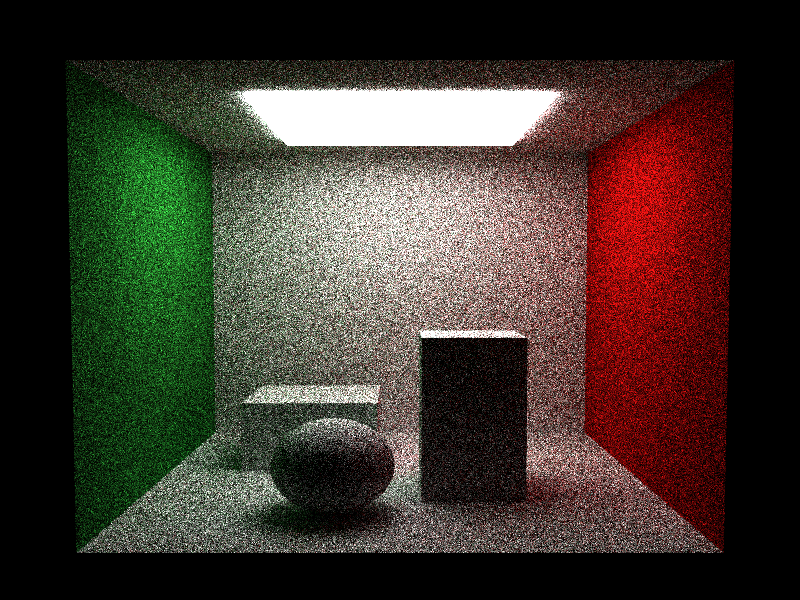
\includegraphics[width=0.92\linewidth]{../out/proj2/req1/proj2_req1_lambert_basic_20260606_151600/render.png}
\caption{Cornell Box difusa, amostragem por BSDF (800$\times$600, SPP=32, seed=42).}
\end{figure}
\figcmd{python -m path_tracing.scripts.proj2_req1_lambert_basic --spp 32 --depth 8 --seed 42 --width 800 --height 600}

\noindent\textbf{Variações de parâmetros} (estudo de ruído$\times$SPP e de profundidade):
\begin{itemize}\small\setlength{\itemsep}{1pt}
\item Convergência: \texttt{-{}-spp 4}, \texttt{16}, \texttt{64}, \texttt{256} (com \texttt{-{}-depth 6 -{}-seed 42}) --- o ruído decai $\propto 1/\sqrt{N}$.
\item Profundidade do caminho: \texttt{-{}-depth 2}, \texttt{4}, \texttt{8} (com \texttt{-{}-spp 64}) --- evidencia o \emph{bleeding} indireto a partir do 4\textsuperscript{o} vértice.
\end{itemize}

\subsection{NEE (Etapa 03)}
\begin{figure}[!ht]
\centering
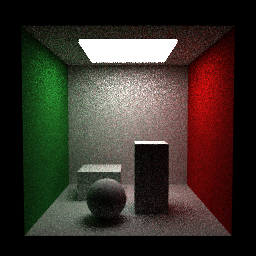
\includegraphics[width=0.92\linewidth]{../out/proj2/req2/proj2_req2_nee_only_20260606_155653/render.png}
\caption{NEE --- execução~1 (256$\times$256, SPP=16, seed=42, $\approx$1{,}89 min): amostragem direta da luz, menor variância que BSDF-only.}
\end{figure}
\begin{figure}[!ht]
\centering
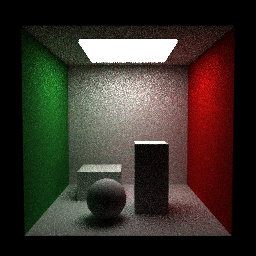
\includegraphics[width=0.92\linewidth]{../out/proj2/req2/proj2_req2_nee_only_20260606_162251/render.png}
\caption{NEE --- execução~2 (256$\times$256, SPP=16, seed=42, $\approx$1{,}99 min): consistência entre runs demonstra reprodutibilidade do estimador.}
\end{figure}
\figcmd{python -m path_tracing.scripts.proj2_req2_nee --spp 16 --depth 8 --seed 42}

\noindent\textbf{Variações de parâmetros} (mesma cena/SPP/semente, dois estimadores):
\begin{itemize}\small\setlength{\itemsep}{1pt}
\item \texttt{-{}-mode bsdf\_only -{}-spp 16 -{}-seed 42} --- alta variância (luz raramente amostrada pela BSDF).
\item \texttt{-{}-mode nee\_only -{}-spp 16 -{}-seed 42} --- amostragem direta: ruído visivelmente menor.
\end{itemize}

\subsection{MIS (Etapa 04)}
\begin{figure}[!ht]
\centering
\includegraphics[width=0.92\linewidth]{../out/proj2/req3/proj2_req3_mis_20260606_161743/render.png}
\caption{MIS (heurística de potência $\beta=2$) combinando BSDF e NEE.}
\end{figure}
\figcmd{python -m path_tracing.scripts.proj2_req3_mis --spp 16 --depth 8 --seed 42}

\noindent\textbf{Variações de parâmetros} (os três estimadores convergem à mesma média --- não-viés):
\begin{itemize}\small\setlength{\itemsep}{1pt}
\item \texttt{-{}-mode bsdf\_only -{}-spp 32 -{}-seed 42}
\item \texttt{-{}-mode nee\_only -{}-spp 32 -{}-seed 42}
\item \texttt{-{}-mode mis -{}-spp 32 -{}-seed 42} --- menor variância combinando ambas as estratégias.
\end{itemize}

\subsection{Roleta Russa (Etapa 05)}
\begin{figure}[!ht]
\centering
\includegraphics[width=0.92\linewidth]{../out/proj2/req5/proj2_req5_mis_no_rr_20260606_163937/render.png}
\caption{MIS \textbf{sem} Roleta Russa (256$\times$256, SPP=16, seed=42): referência de variância para comparação.}
\end{figure}
\begin{figure}[!ht]
\centering
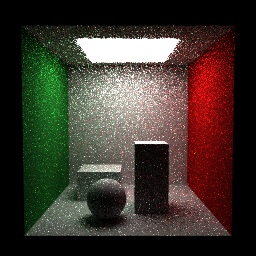
\includegraphics[width=0.92\linewidth]{../out/proj2/req5/proj2_req5_mis_rr_20260606_164126/render.png}
\caption{MIS \textbf{com} Roleta Russa (256$\times$256, SPP=16, seed=42): mesma média, menor custo em caminhos profundos.}
\end{figure}
\begin{figure}[!ht]
\centering
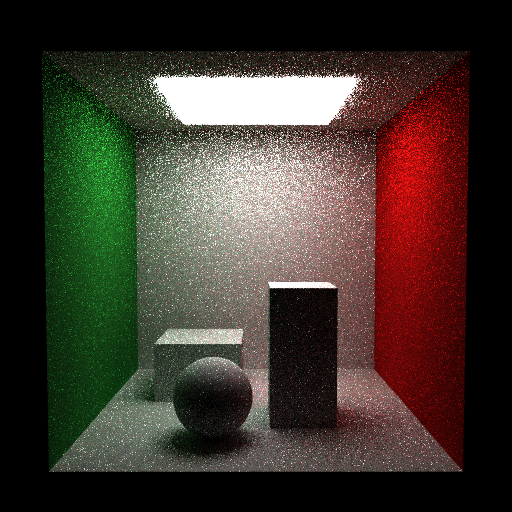
\includegraphics[width=0.92\linewidth]{../out/proj2/req5/proj2_req5_mis_no_rr_20260607_153507/render.png}
\caption{MIS + RR com profundidade mínima~4 (512$\times$512, SPP=12, $\approx$7{,}5 min), gerado com \texttt{-{}-use-rr 4}: maior resolução evidencia a uniformidade da convergência.}
\end{figure}
\figcmd{python -m path_tracing.scripts.proj2_req5_rr --spp 12 --depth 8 --mode mis --use-rr 4}

\noindent\textbf{Variações de parâmetros} (controle off$\times$on e ganho em caminhos profundos):
\begin{itemize}\small\setlength{\itemsep}{1pt}
\item \texttt{-{}-mode mis -{}-use-rr false -{}-spp 32} vs.\ \texttt{-{}-use-rr true -{}-spp 32} --- mesma média, menor tempo.
\item \texttt{-{}-depth 12 -{}-use-rr true} --- a Roleta Russa encurta caminhos longos sem viés.
\item \texttt{-{}-use-rr true -{}-rr-min-depth 6} --- adia a terminação probabilística.
\end{itemize}

\subsection{Luz como malha de triângulos (Etapa 06)}

A cena (\path{src/path_tracing/scenes/cornell_mesh_light.py}) substitui a \texttt{RectAreaLight}
retangular por uma \texttt{TriangleMeshLight}: uma malha de triângulos (octaedro com 8 faces
e raio~0,60) suspensa no teto que serve exclusivamente como fonte NEE\@. A amostragem sorteia
um triângulo com probabilidade proporcional à sua área (via CDF) e sorteia um ponto por
coordenadas baricêntricas uniformes (\path{src/path_tracing/sampling.py},
\texttt{uniform\_triangle}). A geometria emissiva do octaedro é de pequena escala nesta cena
--- sua representação visual é melhor apreciada na cena integrada da
Seção~\ref{sec:showcase}.

Parâmetros do script (\path{src/path_tracing/scripts/proj2_req6_mesh_lights.py}):
\texttt{-{}-mode \{bsdf\_only|nee\_only|mis\}} (integrador),
\texttt{-{}-use-rr \{true|false\}} (Roleta Russa),
\texttt{-{}-spp N} (amostras/pixel),
\texttt{-{}-depth D} (profundidade máxima; mín=4),
\texttt{-{}-width/-{}-height} (resolução),
\texttt{-{}-seed S} (reprodutibilidade).

\begin{figure}[!ht]
\centering
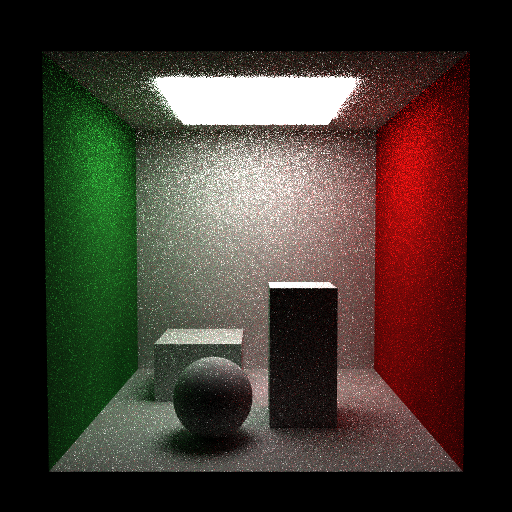
\includegraphics[width=0.92\linewidth]{../out/proj2/req6/proj2_req6_mis_no_rr_20260606_205410/render.png}
\caption{Cornell Box com \texttt{TriangleMeshLight} (octaedro NEE), modo MIS sem RR
(512$\times$512, SPP=16, $\approx$9{,}6 min). A fonte de malha triangular substitui a
\texttt{RectAreaLight}; a redução de variância em relação ao modo \texttt{bsdf\_only} evidencia
o ganho da amostragem direta.}
\end{figure}
\figcmd{python -m path_tracing.scripts.proj2_req6_mesh_lights --spp 16 --depth 8 --mode mis --width 512 --height 512}

\noindent\textbf{Variações de parâmetros}:
\begin{itemize}\small\setlength{\itemsep}{1pt}
\item \texttt{-{}-mode bsdf\_only -{}-spp 16} vs.\ \texttt{-{}-mode mis -{}-spp 16} --- a fonte menor (octaedro) amplifica o ganho relativo do NEE\@.
\item \texttt{-{}-mode mis -{}-use-rr true -{}-spp 32} --- combina amostragem de malha triangular e Roleta Russa.
\end{itemize}

\subsection{Dielétrico (Etapa 07)}

Parâmetros do script (\path{src/path_tracing/scripts/proj2_req7_dielectric.py}):
\texttt{-{}-material \{glass|water\}} (IOR=1{,}5 ou 1{,}33),
\texttt{-{}-absorption R G B} (coeficiente $\sigma$ Beer-Lambert por canal~RGB; \texttt{0 0 0} = incolor; ex.: \texttt{0.2 0.6 1.2} para vidro âmbar absorvendo azul, \texttt{0.30 0.05 0.10} para água azul-esverdeada absorvendo vermelho),
\texttt{-{}-mode \{bsdf\_only|nee\_only|mis\}},
\texttt{-{}-use-rr}, \texttt{-{}-spp}, \texttt{-{}-depth}, \texttt{-{}-width/-{}-height}, \texttt{-{}-seed}.

\paragraph{Vidro incolor (IOR=1{,}5).}
\begin{figure}[!ht]
\centering
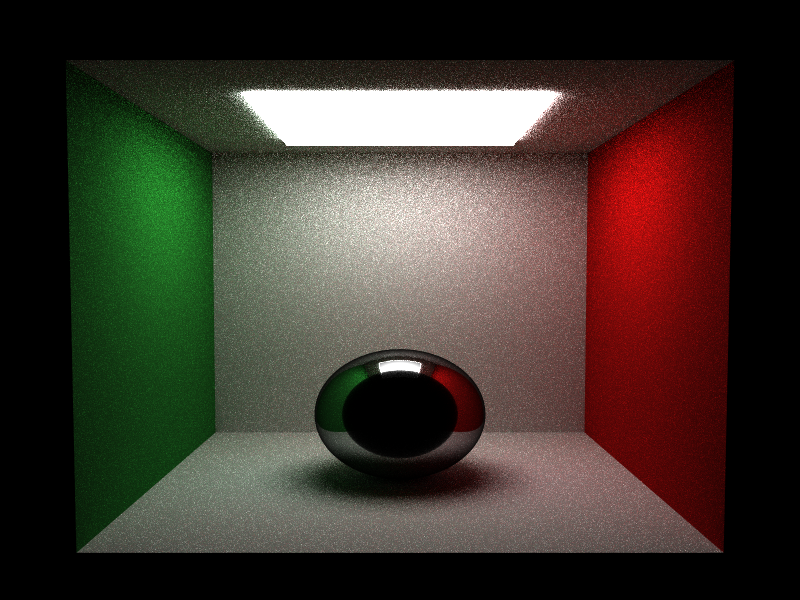
\includegraphics[width=0.92\linewidth]{../out/proj2/req7/proj2_req7_glass_mis_no_rr_20260606_172940/render.png}
\caption{Esfera de vidro incolor (\texttt{DielectricBSDF}, IOR=1{,}5), MIS sem RR (800$\times$600, SPP=64, seed=42, $\approx$58 min). A alta reflectância Fresnel em ângulos rasantes confere aparência especular às bordas; refração de Snell e reflexão interna total (TIR) são observáveis na região central.}
\end{figure}
\begin{figure}[!ht]
\centering
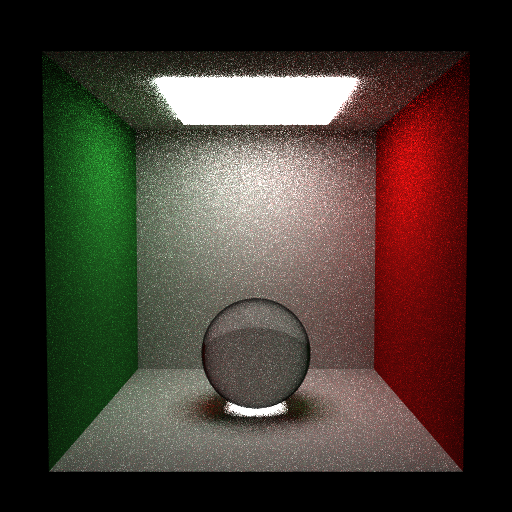
\includegraphics[width=0.92\linewidth]{../out/proj2/req7/proj2_req7_glass_mis_no_rr_20260606_200923/render.png}
\caption{Esfera de vidro incolor (\texttt{DielectricBSDF}, IOR=1{,}5), MIS sem RR (512$\times$512, SPP=32, $\approx$16 min): resolução intermediária; padrão de cáusticas visível no chão.}
\end{figure}
\figcmd{python -m path_tracing.scripts.proj2_req7_dielectric --material glass --spp 64 --depth 8 --mode mis --seed 42 --width 800 --height 600}

\paragraph{Água com absorção de Beer-Lambert (IOR=1{,}33).}
\begin{figure}[!ht]
\centering
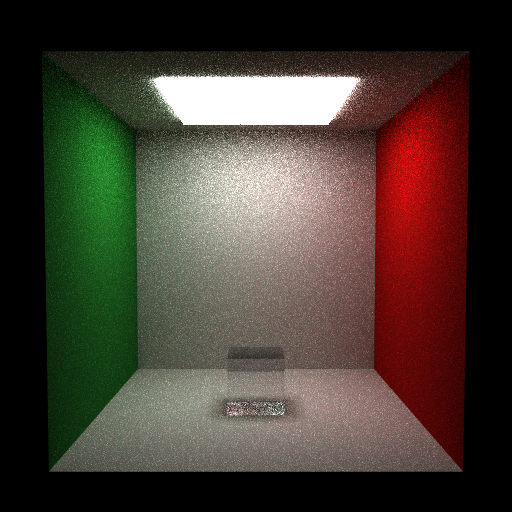
\includegraphics[width=0.92\linewidth]{../out/proj2/req7/proj2_req7_water_mis_no_rr_20260606_204425/render.png}
\caption{Água (IOR=1{,}33), absorção cromática, MIS sem RR (512$\times$512, SPP=64, $\approx$33 min): coloração azul-esverdeada por atenuação seletiva do vermelho.}
\end{figure}
\begin{figure}[!ht]
\centering
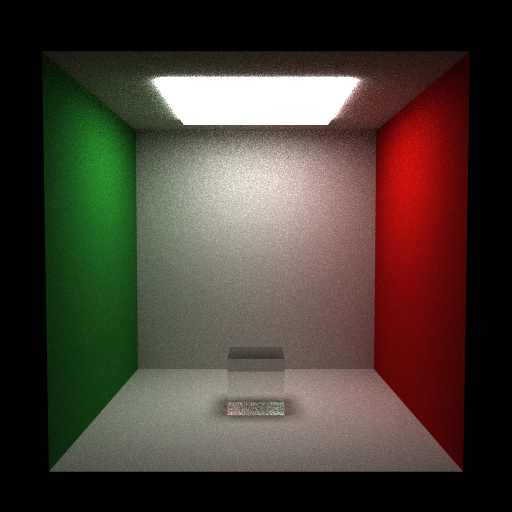
\includegraphics[width=0.92\linewidth]{../out/proj2/req7/proj2_req7_water_mis_no_rr_20260606_212027/render.png}
\caption{Água (IOR=1{,}33), absorção cromática, MIS sem RR (512$\times$512, SPP=256, $\approx$142 min): convergência quase total, ruído praticamente eliminado.}
\end{figure}
\figcmd{python -m path_tracing.scripts.proj2_req7_dielectric --material water --spp 64 --depth 8 --mode mis}

\paragraph{Showcase multi-material dielétrico.}
A cena \path{src/path_tracing/scenes/cornell_dielectric_multi.py} instancia quatro esferas
(\texttt{DielectricBSDF}, raio=0{,}75) dispostas em grade~2$\times$2 no piso da Cornell Box,
cobrindo o espaço de variações de IOR e absorção de Beer-Lambert:

\begin{center}\small
\begin{tabular}{llll}
\textbf{Posição} & \textbf{IOR} & \textbf{Absorção $\sigma$ (RGB)} & \textbf{Efeito visual} \\
\hline
Frente-esq. & 1{,}5 & $(0,0,0)$ incolor & reflexão Fresnel + refração \\
Frente-dir. & 1{,}5 & $(0{,}2,\,0{,}6,\,1{,}2)$ & tom âmbar (absorve azul) \\
Fundo-esq.  & 1{,}33 & $(0,0,0)$ incolor & água incolor, Fresnel suave \\
Fundo-dir.  & 1{,}33 & $(0{,}30,\,0{,}05,\,0{,}10)$ & água azul-esverdeada (absorve vermelho) \\
\end{tabular}
\end{center}

\figmaybe{../out/proj2/req7_dielectric_showcase/proj2_req7_dielectric_showcase_mis_no_rr.png}{Showcase multi-material dielétrico, MIS sem RR (512$\times$512, SPP=32): quatro esferas com \texttt{DielectricBSDF} em variações de IOR ($1{,}5$ / $1{,}33$) e absorção Beer-Lambert, numa Cornell Box com iluminação retangular.}
\figcmd{python -m path_tracing.scripts.proj2_req7_dielectric_showcase --spp 32 --depth 8 --mode mis}

\noindent\textbf{Variações de parâmetros} (material $\times$ absorção $\times$ estimador):
\begin{itemize}\small\setlength{\itemsep}{1pt}
\item \texttt{-{}-material glass -{}-spp 32 -{}-mode mis} (incolor) vs.\ \texttt{-{}-absorption 0.2 0.6 1.2} (âmbar, absorve azul).
\item \texttt{-{}-material water -{}-spp 32 -{}-mode mis} (incolor) vs.\ \texttt{-{}-absorption 0.30 0.05 0.10} (azul-esverdeado, absorve vermelho).
\item \texttt{-{}-material glass -{}-mode bsdf\_only} (cáusticas ruidosas) vs.\ \texttt{-{}-mode mis}.
\item \texttt{-{}-material glass -{}-use-rr true -{}-depth 12} --- caminhos internos profundos (múltiplas reflexões/TIR) com RR.
\end{itemize}

\subsection{Cena integrada (\emph{showcase})}
\label{sec:showcase}

A cena \emph{wall lights} (\path{src/path_tracing/scenes/cornell_wall_lights.py}) reúne numa
Cornell Box todos os recursos implementados no projeto: \textbf{três} fontes de área
(\texttt{RectAreaLight} branca no teto~+ dois painéis hexagonais emissivos nas paredes
laterais, verde à esquerda e vermelho à direita), exercitando NEE com múltiplas fontes de
geometria distinta; duas esferas dielétricas --- vidro incolor (IOR=1{,}5) e âmbar com
absorção de Beer-Lambert; uma esfera difusa azul (\emph{color bleeding}); e duas caixas
Lambertianas rotacionadas. A amostragem de pixel é estratificada (\texttt{stratified}) e a
profundidade máxima é 12.

O script (\path{src/path_tracing/scripts/proj2_showcase_wall_lights.py}) renderiza os quatro
modos do \texttt{PathIntegrator} e grava cópias estáveis em
\path{out/proj2/showcase\_wall\_lights/}.

\figcmd{python -m path_tracing.scripts.proj2_showcase_wall_lights --spp 64 --depth 12 --all}

\noindent Equivalente, modo a modo:
\begin{itemize}\small\setlength{\itemsep}{1pt}
\item \texttt{-{}-mode bsdf\_only -{}-spp 64 -{}-depth 12}
\item \texttt{-{}-mode nee\_only -{}-spp 64 -{}-depth 12}
\item \texttt{-{}-mode mis -{}-spp 64 -{}-depth 12}
\item \texttt{-{}-mode mis -{}-use-rr true -{}-spp 64 -{}-depth 12} (Roleta Russa)
\end{itemize}

\figmaybe{../out/proj2/showcase_wall_lights/proj2_showcase_wall_lights_bsdf_only_no_rr.png}{Showcase --- \texttt{bsdf\_only} (512$\times$512, SPP=64, estratificado, depth=12, $\approx$42 min): alta variância; as fontes hexagonais laterais são raramente amostradas por BSDF puro.}
\figmaybe{../out/proj2/showcase_wall_lights/proj2_showcase_wall_lights_nee_only_no_rr.png}{Showcase --- \texttt{nee\_only} (512$\times$512, SPP=64, estratificado, depth=12, $\approx$100 min): amostragem direta das três fontes (teto + paredes laterais); iluminação direta nítida.}
\figmaybe{../out/proj2/showcase_wall_lights/proj2_showcase_wall_lights_mis_no_rr.png}{Showcase --- \texttt{mis} (512$\times$512, SPP=64, estratificado, depth=12, $\approx$102 min): combina BSDF e NEE com heurística de potência ($\beta=2$); menor variância em superfícies difusas e especulares.}
\figmaybe{../out/proj2/showcase_wall_lights/proj2_showcase_wall_lights_mis_rr.png}{Showcase --- \texttt{mis} + Roleta Russa (512$\times$512, SPP=64, estratificado, depth=12, $\approx$70 min): mesma média, terminação probabilística de caminhos profundos.}

\subsection{Cena combinada (\emph{combined showcase})}
\label{sec:combined-showcase}

A cena \path{src/path_tracing/scenes/cornell_combined_showcase.py} funde as duas cenas anteriores
numa Cornell Box única que exercita simultaneamente todos os recursos implementados:
\textbf{três} fontes de luz (\texttt{RectAreaLight} branca no teto + dois \texttt{TriangleMeshLight}
hexagonais nas paredes, verde e vermelho), \textbf{quatro} esferas \texttt{DielectricBSDF} com
variações de IOR e absorção Beer-Lambert (duas no piso e duas suspensas em alturas distintas),
duas caixas Lambertianas rotacionadas e uma esfera difusa azul para \emph{color bleeding}.

\begin{center}\small
\begin{tabular}{lllll}
\textbf{Objeto} & \textbf{Posição (x,y,z)} & \textbf{r} & \textbf{IOR} & \textbf{Absorção / material} \\
\hline
Esfera piso-esq. & (1.50, 0.80, 3.40) & 0.80 & 1{,}5 & incolor \\
Esfera piso-dir. & (3.90, 0.80, 3.60) & 0.80 & 1{,}5 & âmbar $(0{,}2,\,0{,}6,\,1{,}2)$ \\
Esfera susp.-esq. & (1.40, 3.60, 2.00) & 0.75 & 1{,}33 & água incolor \\
Esfera susp.-dir. & (4.10, 2.60, 2.20) & 0.75 & 1{,}33 & água azul-esverdeada \\
Esfera difusa azul & (2.70, 0.55, 4.70) & 0.55 & — & \texttt{LambertianBSDF} \\
\end{tabular}
\end{center}

\paragraph{Por que regiões das esferas dielétricas aparecem escuras.}
O \texttt{DielectricBSDF} é uma \emph{delta distribution} (\texttt{is\_specular = True}):
em cada vértice o integrador escolhe estocasticamente refletir \emph{ou} refratar, sem
avaliar NEE/MIS naquele bounce. Dois fenômenos produzem escuridão localizada:

\begin{enumerate}\small\setlength{\itemsep}{1pt}
\item \textbf{Caminhos aprisionados (\emph{depth} esgotado).} Um raio que entra na esfera
  realiza pelo menos dois bounces especulares (entrada e saída via Snell). Para esferas
  suspensas, o raio de saída pode atingir outra esfera dielétrica, multiplicando os bounces.
  Se \texttt{max\_depth} for atingido antes de o caminho alcançar uma superfície difusa,
  o integrador retorna radiância zero --- região preta. Aumentar \texttt{--depth} (12 ou mais)
  reduz esse efeito.

\item \textbf{Reflexão interna total (TIR).} Em ângulos acima do ângulo crítico
  $\theta_c = \arcsin(1/\eta)$ (para IOR=1{,}5: $\theta_c \approx 41{,}8°$), o
  \texttt{DielectricBSDF} reflete $100\%$ da energia --- nenhum raio sai do meio. Múltiplas
  TIR consecutivas criam anéis escuros na silhueta da esfera, efeito fisicamente correto
  mas visualmente não intuitivo em baixo SPP.
\end{enumerate}

\noindent Para um render convergido recomenda-se SPP$\,\geq 64$, \texttt{--depth 12} e modo
\texttt{mis}; a Roleta Russa (\texttt{--use-rr true}) acelera o término de caminhos de baixo
\emph{throughput} sem introduzir viés.

\figmaybe{../out/proj2/showcase_combined/proj2_showcase_combined_bsdf_only_no_rr.png}{Cena combinada, \texttt{bsdf\_only} (512$\times$512, SPP=2, estratificado, depth=4): alta variância; esferas dielétricas com regiões escuras por \emph{depth} esgotado e TIR.}
\figmaybe{../out/proj2/showcase_combined/proj2_showcase_combined_nee_only_no_rr.png}{Cena combinada, \texttt{nee\_only} (512$\times$512, SPP=2, estratificado, depth=4): iluminação direta das três fontes nítida nas superfícies difusas; esferas especulares ainda ruidosas pois NEE é pulado em bounces dielétricos (\texttt{is\_specular}).}
\figmaybe{../out/proj2/showcase_combined/proj2_showcase_combined_mis_no_rr.png}{Cena combinada, \texttt{mis} (512$\times$512, SPP=64, estratificado, depth=12): combina BSDF e NEE com heurística de potência ($\beta=2$); menor variância nas superfícies difusas e especulares; regiões TIR ainda visíveis nas bordas das esferas.}
\figmaybe{../out/proj2/showcase_combined/proj2_showcase_combined_mis_rr.png}{Cena combinada, \texttt{mis} + Roleta Russa (512$\times$512, SPP=64, estratificado, depth=12): terminação probabilística de caminhos de baixo \emph{throughput}; reduz tempo de render mantendo estimador não-viesado.}
\figcmd{python -m path_tracing.scripts.proj2_showcase_combined --spp 64 --depth 12 --all}

% =====================================================================
\section{Comparação: Ray Tracing (Projeto 1) \texorpdfstring{$\times$}{x} Path Tracing (Projeto 2)}
\label{sec:comparacao}

A transição do Projeto~1 para o Projeto~2 é, sobretudo, uma \textbf{reescrita do integrador},
não da geometria: câmera \emph{pinhole}, interseções, instanciação e BVH são reaproveitadas. O
ray tracer recursivo (\emph{Whitted}) em \path{src/ray_tracing_2/} avalia Phong analiticamente
e dispara raios secundários apenas para reflexão/refração especular; o path tracer em
\path{src/path_tracing/} estima a equação de transporte de luz~\citep{kajiya1986rendering}
por Monte Carlo, construindo caminhos completos com \emph{throughput} $\beta$
\pbrtsecs{13.1, 13.3, 13.4}.

\subsection{Evolução do material dielétrico}
\label{sec:dielectric-evol}

O material refrativo é o caso mais ilustrativo da evolução. No Projeto~1,
\texttt{TransparentMaterial} (\path{src/ray_tracing_2/material.py}, linha~176) é um material
\emph{recursivo} derivado de Phong: usa Fresnel-Schlick, \texttt{glm.refract()} e atenuação de
Beer-Lambert aplicada nos \emph{raios de sombra}. No Projeto~2, \texttt{DielectricBSDF}
(\path{src/path_tracing/bsdf/dielectric.py}) é uma BSDF \emph{delta} amostrada
estocasticamente, com Fresnel exato e absorção rastreada no integrador. A
Tabela~\ref{tab:dielectric-evol} resume as diferenças.

\paragraph{Limites declarados.} A implementação é em Python puro (\texttt{pyglm}/PIL),
priorizando clareza e corretude; resoluções $\le 512^2$ e SPP moderado são o regime prático.
O dielétrico assume meio \emph{não aninhado} (um nível dentro/fora), suficiente para
esfera/cubo convexos isolados, e omite o fator de radiância $1/\eta^2$ por cancelar em objeto
fechado. \emph{Não} foram implementadas (ficam como evolução): microfacetas GGX, luz infinita/
\emph{environment}, traçado bidirecional (BDPT) e Metropolis (MLT); como os extras já
realizados excedem a cota de pontos de extensão, essas ausências não comprometem o enunciado.

% =====================================================================
\section{Conclusão e Trabalhos Futuros}
\label{sec:conclusao}

Apresentou-se um \emph{path tracer} unidirecional correto, com NEE, MIS, Roleta Russa, luzes
de área (retangular e poliédrica) e materiais dielétricos completos (Snell, Fresnel, TIR e
Beer-Lambert), validados por testes numéricos e por convergência cruzada entre estimadores.
Como trabalhos futuros, destacam-se BSDFs microfacetadas (Cook-Torrance/GGX
\citep{walter2007microfacet}), luz infinita por \emph{environment map}, e métodos
bidirecionais/MCMC para reduzir o ruído de cáusticas. A base ortonormal local segue
\citet{frisvad2012orthonormal}.

% =====================================================================
\bibliographystyle{apalike-sol}
\bibliography{refs}

\clearpage

\begin{table*}[!ht]
\caption{Comparação conceitual entre o ray tracer recursivo (Projeto~1) e o path tracer (Projeto~2).}
\label{tab:rt-vs-pt}
\centering
\begin{tblr}{
width=\textwidth,
colspec={Q[l,wd=0.20\textwidth] Q[l,wd=0.38\textwidth] Q[l,wd=0.38\textwidth]},
row{1}={font=\bfseries},
rows={valign=t},
cells={font=\small}
}
Aspecto & Projeto 1 --- Ray Tracing (Whitted) & Projeto 2 --- Path Tracing \\
Equação resolvida & Phong analítico + reflexão/refração recursiva & Estimador de Monte Carlo da LTE / integral de caminhos~\citep{kajiya1986rendering} \\
Iluminação direta & \texttt{direct\_lighting()} analítico por luz pontual/área & NEE (amostragem da luz) + MIS no último segmento \\
Iluminação indireta & Apenas especular (reflexão/refração) & Difusa e especular (GI completa) via $\beta$ acumulado \\
Sombreamento & Função fechada do material (Phong) & Probabilístico: $\beta \mathrel{\ast}= f\,\lvert\cos\theta\rvert/p$ \\
Terminação & \texttt{can\_spawn\_ray()} / \texttt{max\_depth} fixo & \texttt{min\_depth}=4 + Roleta Russa \pbrtsec{2.2.4} \\
Convergência & Determinística (nítida em baixo SPP) & Estocástica, ruído $\propto 1/\sqrt{N}$ \\
Especular + luz & Reflexão/refração somadas na recursão & Delta: pula NEE/MIS, peso 1 (\texttt{is\_specular}) \\
\end{tblr}
\end{table*}

\begin{table*}[!ht]
\caption{Evolução da implementação dielétrica: ray tracer (Projeto~1) $\times$ path tracer (Projeto~2).}
\label{tab:dielectric-evol}
\centering
\begin{tblr}{
width=\textwidth,
colspec={Q[l,wd=0.20\textwidth] Q[l,wd=0.38\textwidth] Q[l,wd=0.38\textwidth]},
row{1}={font=\bfseries},
rows={valign=t},
cells={font=\small}
}
Aspecto & \texttt{TransparentMaterial} (P1) & \texttt{DielectricBSDF} (P2) \\
Fresnel & Aproximação de Schlick $R_0+(1-R_0)(1-\cos\theta)^5$ & Exato não polarizado $F=\tfrac12(r_\parallel^2+r_\perp^2)$ \pbrtsec{9.5} \\
Reflexão vs.\ refração & Ponderação determinística ($R$ e $1-R$) na recursão & Escolha estocástica (uma direção delta por vértice) \\
Direção refratada & \texttt{glm.refract()} & Forma vetorial no frame da normal geométrica \\
Reflexão interna total & Teste heurístico sobre a direção refratada & Analítico: $\sin^2\theta_t = \eta^2(1-\cos^2\theta_i)\ge 1$ \\
Entrada/saída do meio & \texttt{front\_face}/\texttt{backfacing} (normal virada) & Sinal de $\omega_o\!\cdot\! n$ (normal geométrica) \\
Absorção (Beer-Lambert) & Nos raios de sombra ao sair do meio \pbrtsec{11.2} & Rastreio de meio: $\beta\mathrel{\ast}=e^{-\sigma d}$ em qualquer segmento interno \\
Integração com a luz & Embutida no sombreamento recursivo de Phong & Especular pula NEE/MIS (peso 1); GI por amostragem da BSDF \\
\end{tblr}
\end{table*}

% =====================================================================
\section*{Anexo A: Quadro de Referências Conceituais}

O quadro a seguir mapeia cada conceito implementado à evidência mais direta no código
(\path{src/path_tracing/}) e a uma nota compacta com as páginas dos slides, a seção mais
próxima em \pbrtbook{} e as linhas de código relevantes.

\begin{table*}[!ht]
\caption{Mapeamento conceito $\to$ evidência $\to$ referências (etapas 02--07 e infraestrutura).}
\label{tab:referencias}
\centering
\begin{tblr}{
width=\textwidth,
colspec={Q[l,wd=0.24\textwidth] Q[l,wd=0.34\textwidth] Q[l,wd=0.36\textwidth]},
row{1}={font=\bfseries},
rows={valign=t},
cells={font=\small}
}
Conceito de referência & Evidência principal & Nota \\
Núcleo unidirecional e \emph{throughput} $\beta$ & \texttt{PathIntegrator}, \texttt{Li()} & \slidesref{inf2608slides08}{8}{—}; \pbrtsec{13.3}; \ghsrclines{integrators/path_tracer.py}{31,68}. \\
BSDF Lambertiana e método de Malley & \texttt{LambertianBSDF.eval/sample/pdf}, \texttt{cosine\_hemisphere()} & \slidesref{inf2608slides07}{7}{—}; \pbrtsecpair{9.2}{A.5}; \ghsrclines{bsdf/lambertian.py}{17,45,73}; \ghsrclines{sampling.py}{61}. \\
Base ortonormal local (Frisvad) & \texttt{ONB}, \texttt{frisvad\_branchless()} & \slidesref{inf2608slides09}{9}{—}; \citet{frisvad2012orthonormal}; \ghsrclines{onb.py}{15,60}. \\
NEE: conversão área $\to$ ângulo sólido & \texttt{RectAreaLight.sample\_Li/pdf\_Li}, laço NEE & \slidesref{inf2608slides09}{9}{—}; \pbrtsecpair{12.4}{12.6}; \ghsrclines{lights/area_rect.py}{65,111}; \ghsrclines{integrators/path_tracer.py}{178}. \\
MIS (heurística de potência $\beta=2$) & \texttt{balance\_heuristic}, \texttt{power\_heuristic} & \slidesref{inf2608slides09}{9}{—}; \pbrtsec{2.2.3}; \citet{veach1995optimallycombin}; \ghsrclines{mis.py}{16,45}. \\
Roleta Russa (não-viesada) & terminação probabilística por $\beta$ & \slidesref{inf2608slides09}{9}{—}; \pbrtsec{2.2.4}; \citet{misso2022unbiased}; \ghsrclines{integrators/path_tracer.py}{274}. \\
Luz poliédrica (uniforme por área) & \texttt{TriangleMeshLight.sample\_Li/pdf\_Li}, \texttt{uniform\_triangle()} & \slidesref{inf2608slides09}{9}{—}; \pbrtsec{6.5}; \ghsrclines{lights/area_mesh.py}{22,95,163}; \ghsrclines{sampling.py}{93}. \\
Dielétrico: Snell, Fresnel, TIR & \texttt{DielectricBSDF.sample}, \texttt{is\_specular} & \pbrtsec{9.5}; \ghsrclines{bsdf/dielectric.py}{29,71,75,112}. \\
Beer-Lambert (rastreio de meio) & atenuação $e^{-\sigma d}$ no integrador & \pbrtsec{11.2}; \ghsrclines{integrators/path_tracer.py}{118}. \\
Câmera, filme e amostragem de pixel & \texttt{Camera.generate\_ray()}, \texttt{Film.get\_samples\_for\_pixel/render} & \slidesref{inf2608slides07}{7}{—}; \ghsrclines{camera.py}{28}; \ghsrclines{film.py}{104,156}. \\
\end{tblr}
\end{table*}

\end{document}
